%% ============================================================
%%  Parking Operational Intelligence Platform — Final Report
%%  Flipkart Gridlock Challenge · Round 2 · Theme 1
%%
%%  Compiler : pdflatex  (run twice for cross-references)
%%  Required packages: see \usepackage block below
%% ============================================================

\documentclass[12pt,a4paper]{article}

%% --- Core packages ---
\usepackage[T1]{fontenc}
\usepackage[utf8]{inputenc}
\usepackage{lmodern}
\usepackage[margin=2.2cm]{geometry}
%\usepackage{microtype}  %% disabled for compile speed
\usepackage{placeins}
\usepackage{adjustbox}

%% --- Math ---
\usepackage{amsmath,amssymb,amsfonts}
\usepackage{mathtools}

%% --- Tables ---
\usepackage{booktabs}
\usepackage{longtable}
\usepackage{array}
\usepackage{multirow}
\usepackage{makecell}
\usepackage{tabularx}
\usepackage{xcolor}
\usepackage{colortbl}

%% --- Figures & Graphics ---
\usepackage{graphicx}
\usepackage{float}
\usepackage{caption}
\usepackage{subcaption}

%% --- TikZ (for flowcharts) ---
\usepackage{tikz}
\usetikzlibrary{shapes.geometric, shapes.arrows, arrows.meta,
                positioning, fit, backgrounds, calc, shadows.blur,
                decorations.pathreplacing}

%% --- Lists & Enumerations ---
\usepackage{enumitem}

%% --- Hyperlinks ---
\usepackage[colorlinks=true,linkcolor=blue!60!black,
            citecolor=green!50!black,urlcolor=blue!70!black]{hyperref}

%% --- Section formatting ---
\usepackage{titlesec}
\titleformat{\section}{\large\bfseries}{\thesection.}{0.6em}{}[\titlerule]
\titleformat{\subsection}{\normalsize\bfseries}{\thesubsection}{0.5em}{}

%% --- Abstract formatting ---
\usepackage{abstract}
\renewcommand{\abstractnamefont}{\normalfont\bfseries}

%% --- Algorithm / code ---
\usepackage{algorithm}
\usepackage{algpseudocode}

%% --- Two-column for selected tables ---
\usepackage{multicol}

%% ============================================================
%%  COLOUR PALETTE
%% ============================================================
\definecolor{darkblue}{RGB}{15,55,120}
\definecolor{accentblue}{RGB}{30,100,200}
\definecolor{accentgreen}{RGB}{0,128,80}
\definecolor{accentorange}{RGB}{200,90,0}
\definecolor{accentred}{RGB}{180,30,30}
\definecolor{lightgray}{RGB}{245,245,245}
\definecolor{medgray}{RGB}{180,180,180}
\definecolor{tikzblue}{RGB}{52,120,200}
\definecolor{tikzgreen}{RGB}{40,160,80}
\definecolor{tikzorange}{RGB}{220,110,20}
\definecolor{tikzred}{RGB}{200,40,40}
\definecolor{tikzpurple}{RGB}{120,40,180}

%% ============================================================
%%  FIGURE PLACEHOLDER COMMAND
%%  Usage: %% Removed placeholder label
%% ============================================================
\newcommand{\figplaceholder}[3]{%
  \begin{figure}[htbp]
    \centering
    \fbox{%
      \begin{minipage}[c][#1][c]{0.92\linewidth}
        \centering
        \textcolor{medgray}{\Large\textit{[Figure: #2]}}\\[4pt]
        \textcolor{medgray}{\small Replace with actual plot image}
      \end{minipage}%
    }
    \caption{#2}
    \label{#3}
  \end{figure}%
}

%% ============================================================
%%  TITLE BLOCK
%% ============================================================
\title{%
  \LARGE\bfseries
  Parking Operational Intelligence Platform:\\
  A Multi-Dimensional Spatial Intelligence Framework\\
  for Urban Enforcement Decision Support\\[6pt]
  \large\normalfont\textit{Flipkart Gridlock Challenge — Round 2, Theme 1}
}

\author{%
  \small Abinash Behera \enspace Ansh Patidar \enspace Sumit Kumar \enspace Tanmay Tiwari%
}

\date{\normalsize June 2026}

%% ============================================================
\begin{document}
%% ============================================================

\maketitle
\thispagestyle{empty}

\begin{abstract}
The Flipkart Gridlock Challenge asked participants to transform large-scale parking violation logs from Bengaluru into actionable enforcement intelligence. A raw violation count is not enough for traffic operations: a two-wheeler parked briefly in a side lane is not operationally equivalent to a truck blocking a junction during peak time. This report presents the Parking Operational Intelligence Platform (POIP), an end-to-end pipeline that converts 298,450 anonymised parking violations into a ranked daily enforcement queue by combining spatial intelligence, parking-risk scoring, hotspot evolution, propagation pressure, archetype discovery, forecasting, semantic search, and graph analytics.

The system is designed for Bengaluru Traffic Police, smart-city teams, GIS teams, dashboard developers, and future research work. The dashboard consumes only exported artifacts; it never retrains models or recomputes scores. The central operational contribution is a dynamic parking-zone governance framework: road segments are treated as adaptive zones whose parking duration, fee level, and enforcement intensity change with congestion risk. The report remains honest about what the data can and cannot prove: the dataset supports hotspot identification, prioritisation, and policy design, but it does not by itself establish causal patrol effects without joined patrol logs.
\end{abstract}

\vspace*{\fill}

\newpage
\tableofcontents
\newpage

%% ============================================================
\section{Introduction}
%% ============================================================

\subsection{Urban Parking Congestion Challenges}

Unregulated parking constitutes one of the most pervasive and measurable contributors to
urban traffic congestion in Indian cities. Unlike highway bottlenecks or signal-timing
failures—both addressed by dedicated infrastructure—illegal parking is a distributed,
dynamic phenomenon that manifests simultaneously across hundreds of locations, varies by
time of day and day of week, and is mediated by the capacity of local enforcement
institutions. A truck illegally parked at a major junction can reduce effective lane
capacity by fifty percent for the duration of its presence; a cluster of vehicles along a
commercial artery during peak hours can cascade into gridlock across multiple adjacent roads.

Traffic police departments in cities such as Bengaluru operate camera-assisted enforcement
systems (e.g., SCITA) that generate geo-tagged violation records in near-real time. The
result is a large-scale, continuously growing log of spatial events. However, the operational
intelligence historically extracted from this log has been limited to frequency counts and
geographic heat maps—neither of which accounts for violation severity, spatial propagation,
temporal persistence, or the institutional capacity of the responding precinct.

\subsection{Limitations of Traditional Enforcement Systems}

A car double-parked at a busy commercial junction during peak hours is not the same as a
truck left on an empty roadside at midnight---yet traditional enforcement systems treat
the second one as a greater offense, ranking locations purely by raw violation count. We set out to address
exactly this gap. Conventional parking enforcement analysis is characterised by four
structural deficiencies we specifically designed the POIP to overcome:

\begin{enumerate}[leftmargin=1.5em]
  \item \textbf{Homogeneous violation treatment.} Existing systems rank locations by raw
  violation count, treating a two-wheeler parked momentarily on a side street identically
  to a tanker blocking a road crossing.

  \item \textbf{Temporal blindness.} Count-based methods aggregate over time windows without
  distinguishing a location with fifty violations on one anomalous day from one that
  consistently records violations across the entire observation period.

  \item \textbf{Spatial independence assumption.} Classical hot-spot methods treat each
  location as independent, ignoring the propagation of congestion through the road network.

  \item \textbf{No institutional capacity modelling.} A location in an overloaded police
  precinct effectively has a lower probability of receiving timely enforcement, regardless
  of violation severity.
\end{enumerate}

\subsection{Motivation}

The central research question is: \textit{How can hundreds of thousands of individually
unremarkable parking violation records be synthesised into a spatially-aware,
temporally-informed, institutionally-grounded priority ranking that guides optimal resource
allocation for traffic enforcement?}

\subsection{Contributions}

This project makes the following primary contributions:

\begin{enumerate}[leftmargin=1.5em]
  \item \textbf{Parking Obstruction Index (POI):} A seven-factor multiplicative composite
  quantifying the true obstructive impact of each violation.

  \item \textbf{Propagation Modelling:} A distance-weighted nearest-neighbour spillover model
  capturing spatial congestion propagation.

  \item \textbf{Enforcement Failure Index (EFI):} A five-component composite identifying
  locations where enforcement is systematically insufficient.

  \item \textbf{Congestion Impact Score (CIS):} A six-component network-aware severity
  composite with operational banding (Low / Medium / High / Critical).

  \item \textbf{Hotspot Lifecycle Taxonomy:} A rule-based six-state temporal trajectory model.

  \item \textbf{Behavioural Archetype Discovery:} Unsupervised identification of six
  operationally distinct hotspot archetypes with tailored intervention strategies.

  \item \textbf{Integrated Priority Engine:} A ten-component weighted rank composite with
  archetype multipliers producing the final enforcement queue.

  \item \textbf{Semantic Search Layer:} Transformer-based natural-language querying of the
  hotspot database.

  \item \textbf{Graph Intelligence Layer:} PageRank-based strategic targeting and community
  detection for district-level resource allocation.
\end{enumerate}

%% ============================================================
\section{Dataset Overview}
%% ============================================================

\subsection{Dataset Description}

The dataset consists of 298,450 anonymised parking violation records collected in Bengaluru,
Karnataka, India, spanning the period January to May. Records were sourced from a
camera-assisted enforcement system and encompass Bengaluru's core urban zones (latitude
$\approx 12.90$--$12.93$°N, longitude $\approx 77.60$--$77.70$°E).

\subsection{Data Characteristics and Quality Assessment}

The raw dataset spans 24 columns covering identifiers, spatial coordinates, timestamps, vehicle attributes, station metadata, and validation fields.

Three columns are entirely null (\texttt{description}, \texttt{closed\_datetime},
\texttt{action\_taken\_timestamp}) and were excluded from all analysis. The
\texttt{data\_sent\_to\_scita\_timestamp} field is 85.87\% absent, indicating partial SCITA
transmission. The \texttt{updated\_vehicle\_type} field (available for $\sim$58\% of records)
was used in preference to the original \texttt{vehicle\_type} wherever available, as it
reflects post-review classification.

\textbf{What the data tells us about current enforcement.} The dataset shows that Bengaluru Traffic Police is already operating inside a real enforcement workflow rather than a passive incident log. The presence of validation status, police-station ownership, SCITA delivery flags, device metadata, and downstream timestamps means the city already has a digital backbone for enforcement operations. What the data does not give us is a direct causal before/after patrol log. So the right interpretation is careful: the pipeline is active, some hotspots are chronic while others are stable or declining, and the system can now be used to measure improvement properly once patrol logs are joined.

%% Removed placeholder fig:missing

%% ============================================================
\section{Proposed Methodology}
%% ============================================================

\subsection{System Overview}

The Parking Operational Intelligence Platform is structured as a sequential analytics
pipeline. Each module produces outputs consumed by subsequent modules, culminating in a
multi-format dashboard export. The system moves from 298,450 individual violation records
through spatial discretisation, severity quantification, network-aware aggregation, temporal
trend analysis, unsupervised behavioural classification, gradient-boosted forecasting, and
composite priority scoring.

\subsection{End-to-End Architecture}

Figure~\ref{fig:architecture} presents the complete system architecture as a sequential
pipeline with 12 processing stages.

%% ============================================================
%%  TIKZ FLOWCHART 1 — SYSTEM ARCHITECTURE
%% ============================================================
\begin{figure}[htbp]
\centering
\resizebox{0.97\textwidth}{!}{%
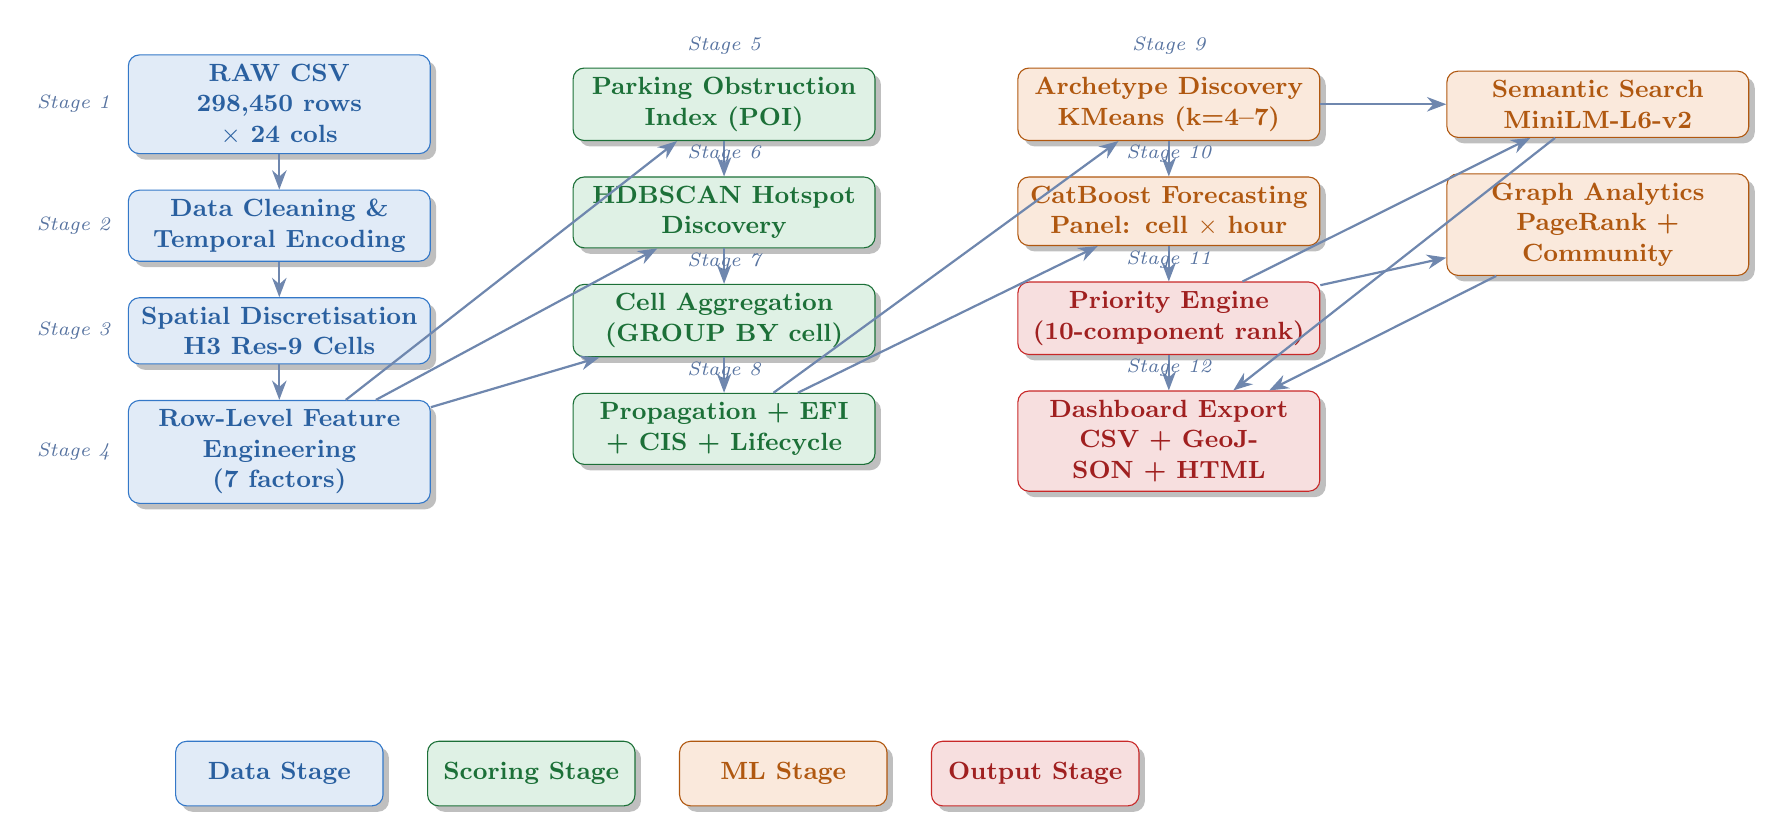
\begin{tikzpicture}[
  node distance = 0.45cm and 0.3cm,
  box/.style    = {rectangle, rounded corners=4pt, minimum width=3.8cm,
                   minimum height=0.82cm, align=center, font=\small\bfseries,
                   drop shadow, text width=3.6cm},
  databox/.style= {box, fill=tikzblue!15, draw=tikzblue, text=tikzblue!80!black},
  scorebox/.style={box, fill=tikzgreen!15, draw=tikzgreen!70!black, text=tikzgreen!70!black},
  mlbox/.style  = {box, fill=tikzorange!15, draw=tikzorange!80!black, text=tikzorange!80!black},
  outbox/.style = {box, fill=tikzred!15, draw=tikzred, text=tikzred!80!black},
  arrow/.style  = {-{Stealth[length=7pt]}, thick, color=darkblue!60},
  label/.style  = {font=\scriptsize\itshape, text=darkblue!70},
]

%% --- Column 1: Data Stages ---
\node[databox] (raw)    {RAW CSV\\298,450 rows $\times$ 24 cols};
\node[databox, below=of raw]  (clean)  {Data Cleaning \&\\Temporal Encoding};
\node[databox, below=of clean](spatial){Spatial Discretisation\\H3 Res-9 Cells};
\node[databox, below=of spatial](feat) {Row-Level Feature\\Engineering (7 factors)};

%% --- Column 2: Scoring Stages ---
\node[scorebox, right=1.8cm of raw]    (poi)   {Parking Obstruction\\Index (POI)};
\node[scorebox, below=of poi]          (hdb)   {HDBSCAN Hotspot\\Discovery};
\node[scorebox, below=of hdb]          (agg)   {Cell Aggregation\\(GROUP BY cell)};
\node[scorebox, below=of agg]          (comp)  {Propagation + EFI\\+ CIS + Lifecycle};

%% --- Column 3: ML + Output Stages ---
\node[mlbox,   right=1.8cm of poi]    (arch)  {Archetype Discovery\\KMeans (k=4--7)};
\node[mlbox,   below=of arch]         (fore)  {CatBoost Forecasting\\Panel: cell $\times$ hour};
\node[outbox,  below=of fore]         (prio)  {Priority Engine\\(10-component rank)};
\node[outbox,  below=of prio]         (dash)  {Dashboard Export\\CSV + GeoJSON + HTML};

%% --- Semantic + Graph (side) ---
\node[mlbox,   right=1.6cm of arch]   (sem)   {Semantic Search\\MiniLM-L6-v2};
\node[mlbox,   below=of sem]          (graph) {Graph Analytics\\PageRank + Community};

%% --- Arrows Col1 ---
\draw[arrow] (raw)    -- (clean);
\draw[arrow] (clean)  -- (spatial);
\draw[arrow] (spatial)-- (feat);

%% --- Arrows Col1 → Col2 ---
\draw[arrow] (feat)   -- (poi);
\draw[arrow] (feat)   -- (hdb);
\draw[arrow] (feat)   -- (agg);

%% --- Arrows Col2 ---
\draw[arrow] (poi)    -- (hdb);
\draw[arrow] (hdb)    -- (agg);
\draw[arrow] (agg)    -- (comp);

%% --- Arrows Col2 → Col3 ---
\draw[arrow] (comp)   -- (arch);
\draw[arrow] (comp)   -- (fore);
\draw[arrow] (arch)   -- (fore);
\draw[arrow] (fore)   -- (prio);
\draw[arrow] (prio)   -- (dash);

%% --- Side modules ---
\draw[arrow] (arch) -- (sem);
\draw[arrow] (prio) -- (sem);
\draw[arrow] (prio) -- (graph);
\draw[arrow] (sem)  -- (dash);
\draw[arrow] (graph)-- (dash);

%% --- Side labels ---
\node[label, left=0.1cm of raw]  {Stage 1};
\node[label, left=0.1cm of clean]{Stage 2};
\node[label, left=0.1cm of spatial]{Stage 3};
\node[label, left=0.1cm of feat] {Stage 4};
\node[label, above=0.05cm of poi]{Stage 5};
\node[label, above=0.05cm of hdb]{Stage 6};
\node[label, above=0.05cm of agg]{Stage 7};
\node[label, above=0.05cm of comp]{Stage 8};
\node[label, above=0.05cm of arch]{Stage 9};
\node[label, above=0.05cm of fore]{Stage 10};
\node[label, above=0.05cm of prio]{Stage 11};
\node[label, above=0.05cm of dash]{Stage 12};

%% --- Legend ---
\begin{scope}[shift={(0,-8.5)}]
  \node[databox, minimum width=2.6cm, text width=2.4cm]  at (0,0)    {Data Stage};
  \node[scorebox, minimum width=2.6cm, text width=2.4cm] at (3.2,0)  {Scoring Stage};
  \node[mlbox,   minimum width=2.6cm, text width=2.4cm]  at (6.4,0)  {ML Stage};
  \node[outbox,  minimum width=2.6cm, text width=2.4cm]  at (9.6,0)  {Output Stage};
\end{scope}

\end{tikzpicture}
}
\caption{End-to-end system architecture of the Parking Operational Intelligence Platform.
         Arrows denote data flow between processing stages.}
\label{fig:architecture}
\end{figure}

%% ============================================================
\subsection{Data Processing and Feature Engineering}

Raw data cleaning involves UTC-aware datetime parsing, numeric coercion for coordinates,
whitespace normalisation for categorical fields, and JSON parsing for the multi-label
violation type field. Records with missing GPS coordinates are excluded, preserving all
298,450 records with valid spatial information.

\paragraph{Temporal encoding.}
Six binary temporal indicators are derived from the creation timestamp:
\texttt{is\_weekend} (Saturday/Sunday), \texttt{is\_morning\_peak} (07:00--10:00),
\texttt{is\_evening\_peak} (17:00--21:00), and \texttt{is\_night} (22:00--05:00), alongside
integer \texttt{hour} and \texttt{day\_of\_week}.

\paragraph{Spatial discretisation.}
Each record is mapped to an H3 resolution-9 hexagonal cell ($\approx$174 m edge length,
$\approx$105,332 m$^2$ area). In the execution environment, H3 was unavailable and a
coordinate-rounding fallback (\texttt{cell\_\{lat3\}\_\{lon3\}}) was employed, producing
cells of equivalent scale.

The engineered features are defined in the score-specific subsections below.

%% ============================================================
\subsection{Parking Obstruction Index (POI)}
%% ============================================================

The Parking Obstruction Index (POI) is the per-violation severity score used throughout the report. It multiplies vehicle footprint, violation severity, junction proximity, density, recurrence, stability, and station burden, then compresses the product with \texttt{log1p} so the scale stays interpretable.

\subsubsection*{Formulation}

The raw POI is the multiplicative product of all seven factors; the final POI applies a
log-transform to compress the extreme right tail:

\begin{equation}
\boxed{
\mathrm{POI} \;=\; \ln\!\Bigl(1 + W_v \cdot W_s \cdot J \cdot D \cdot R \cdot \Sigma \cdot B\Bigr)
}
\label{eq:poi}
\end{equation}

\begin{table}[htbp]
\centering
\caption{POI Component Variables}
\label{tab:poi}
\begin{tabularx}{\textwidth}{@{}clXll@{}}
\toprule
\textbf{Symbol} & \textbf{Feature} & \textbf{Description} & \textbf{Range} & \textbf{Scale}\\
\midrule
$W_v$ & vehicle\_weight   & Obstruction capacity: 1=two-wheeler \ldots{} 5=tanker/bus & \{1,2,3,4,5\}   & Ordinal\\
$W_s$ & severity\_weight  & Max violation severity over label list                    & \{2,3,4,5\}     & Ordinal\\
$J$   & junction\_factor  & 3.0 if named junction; 1.0 otherwise                      & \{1.0, 3.0\}    & Binary\\
$D$   & density\_factor   & cell\_volume / $\overline{\text{cell\_volume}}$, clipped  & [0.5, 3.0]      & Continuous\\
$R$   & recurrence\_factor& Within-hour repeat count binned: ${\le}1\to1.0$; 2-3$\to1.5$; ${>}3\to2.0$ & \{1.0,1.5,2.0\} & Binned\\
$\Sigma$ & stability\_factor & days\_active / median(days\_active), clipped           & [0.5, 3.0]      & Continuous\\
$B$   & station\_burden\_factor & station\_volume / $\overline{\text{station\_volume}}$, clipped & [0.75, 1.5] & Continuous\\
\bottomrule
\end{tabularx}
\end{table}

\paragraph{Why the components matter.}
Vehicle size and violation type capture direct road occupation, while junction proximity, local density, recurrence, hotspot stability, and station burden capture the context around the incident. For multi-label records, the maximum severity label is used because the worst blocking behaviour dominates the operational response. The log transform keeps extreme cases on the same scale as routine violations while preserving rank order.


\subsubsection*{Observed Distribution}

Across all 298,450 records the POI exhibits the following empirical statistics:

\begin{center}
\small
\begin{tabular}{@{}lrrrrrrr@{}}
\toprule
 & \textbf{Mean} & \textbf{Std} & \textbf{Min} & \textbf{Q1} & \textbf{Median} & \textbf{Q3} & \textbf{Max}\\
\midrule
POI & 2.5858 & 1.5042 & 0.3185 & 1.2691 & 2.2447 & 3.7299 & 6.9790\\
\bottomrule
\end{tabular}
\end{center}

The distribution is right-skewed (mean 2.586 $>$ median 2.245): routine violations sit in the middle band, while the upper tail captures the most disruptive events. Table~\ref{tab:poi_bands} gives the operational interpretation.

\begin{table}[htbp]
\centering
\caption{POI Severity Bands and Operational Interpretation}
\label{tab:poi_bands}
\small
\begin{tabularx}{\textwidth}{@{}clp{5.2cm}X@{}}
\toprule
\textbf{POI Range} & \textbf{Severity} & \textbf{Characteristics} & \textbf{Enforcement Response}\\
\midrule
$<1.0$   & Minimal       & Light vehicle, minor violation, low-density non-junction, first occurrence & Observation only\\
1.0--2.0 & Low-Moderate  & Standard car/auto, moderately active non-junction, some intra-day recurrence & Routine patrol; warning\\
2.0--4.0 & Moderate-High & CAR at junction, or heavy vehicle in high-density chronic cell & Active citation; tow-readiness\\
$>4.0$   & Critical      & Heavy vehicle at named junction in chronic, dense, overloaded precinct & Immediate dispatch; tow deployment\\
\bottomrule
\end{tabularx}
\end{table}

%% Removed placeholder fig:poi_dist

%% ============================================================
%%  TIKZ FLOWCHART 2 — POI COMPUTATION
%% ============================================================
\begin{figure}[htbp]
\centering
\resizebox{0.85\textwidth}{!}{%
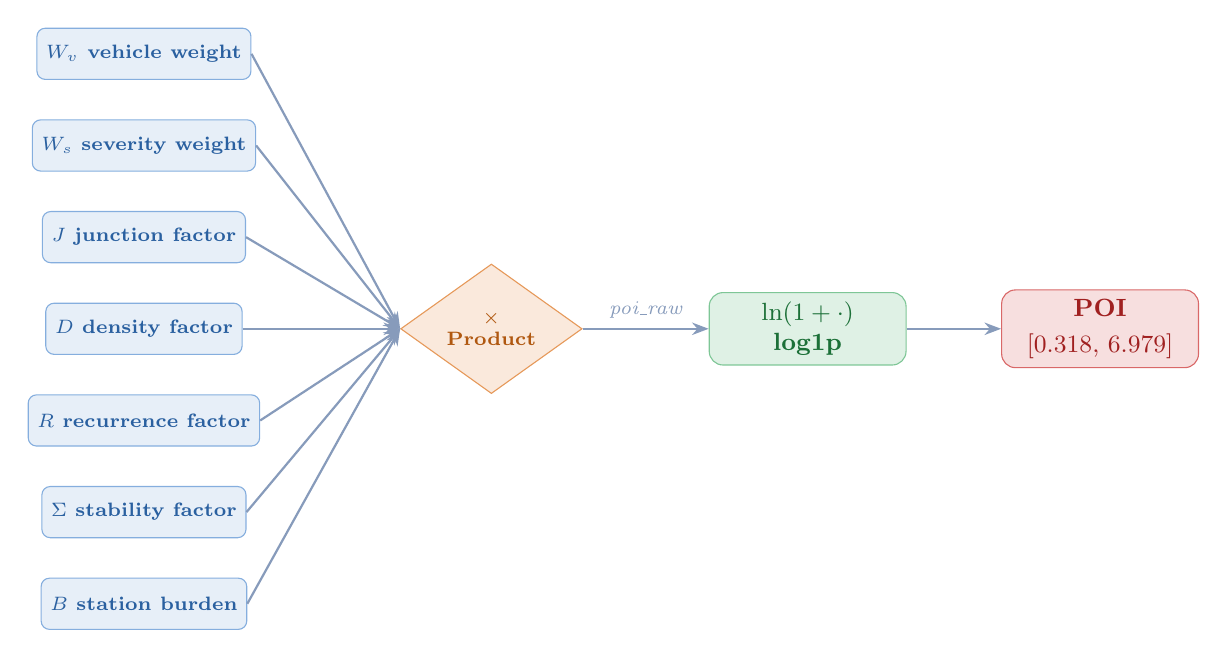
\begin{tikzpicture}[
  node distance = 0.5cm and 0.8cm,
  inpnode/.style   = {rectangle, rounded corners=3pt, fill=tikzblue!12, draw=tikzblue!60,
                  minimum width=2.2cm, minimum height=0.65cm, align=center,
                  font=\scriptsize\bfseries, text=tikzblue!80!black},
  prodnode/.style  = {diamond, fill=tikzorange!15, draw=tikzorange!70, minimum width=2.2cm,
                  minimum height=1.4cm, align=center, font=\scriptsize\bfseries,
                  text=tikzorange!80!black, aspect=1.4},
  lognode/.style   = {rectangle, rounded corners=5pt, fill=tikzgreen!15, draw=tikzgreen!60,
                  minimum width=2.5cm, minimum height=0.72cm, align=center,
                  font=\small\bfseries, text=tikzgreen!70!black},
  outnode/.style = {rectangle, rounded corners=5pt, fill=tikzred!15, draw=tikzred!70,
                  minimum width=2.5cm, minimum height=0.72cm, align=center,
                  font=\small\bfseries, text=tikzred!80!black},
  arr/.style   = {-{Stealth[length=6pt]}, thick, color=darkblue!50},
]

%% Inputs (vertical stack on left)
\node[inpnode] (wv)  {$W_v$ vehicle weight};
\node[inpnode, below=of wv]  (ws)  {$W_s$ severity weight};
\node[inpnode, below=of ws]  (j)   {$J$ junction factor};
\node[inpnode, below=of j]   (d)   {$D$ density factor};
\node[inpnode, below=of d]   (r)   {$R$ recurrence factor};
\node[inpnode, below=of r]   (sig) {$\Sigma$ stability factor};
\node[inpnode, below=of sig] (b)   {$B$ station burden};

%% Product node
\node[prodnode, right=2.0cm of d] (mult) {\textbf{$\times$}\\Product};

%% Log node
\node[lognode, right=1.6cm of mult] (log1p) {$\ln(1 + \cdot)$\\log1p};

%% Output
\node[outnode, right=1.2cm of log1p] (poi) {\textbf{POI}\\[2pt]$[0.318,\,6.979]$};

%% Arrows from inputs to product
\foreach \n in {wv, ws, j, d, r, sig, b} {
  \draw[arr] (\n.east) -- (mult.west);
}

\draw[arr] (mult)  -- node[above,font=\scriptsize\itshape]{$\text{poi\_raw}$} (log1p);
\draw[arr] (log1p) -- (poi);

\end{tikzpicture}
}
\caption{POI computation flow: seven independent factors combined multiplicatively, then
         log1p-transformed to produce the Parking Obstruction Index.}
\label{fig:poi_flow}
\end{figure}

%% ============================================================
\subsection{Spatial Intelligence Framework}
%% ============================================================

H3 resolution-9 hexagonal cells ($\approx$174 m edge length, $\approx$105,332 m$^2$) serve
as the atomic unit of spatial analysis. The cell identifier is computed as:

\begin{verbatim}
  spatial_cell = h3.latlng_to_cell(lat, lon, res=9)
\end{verbatim}

Cell-level aggregation (GROUP BY \texttt{spatial\_cell}) reduces the 298,450-row record
dataset to a compact set of cells, each characterised by 25 aggregated features including
violation counts, POI statistics, vehicle composition ratios, temporal peak ratios, dominant
police station, and computed composite scores.

%% Removed placeholder fig:spatial

%% ============================================================
\subsection{Propagation Modelling}
%% ============================================================

A fundamental limitation of location-level analysis is the assumption of spatial
independence. The propagation score explicitly models congestion spillover from high-severity
cells to their geographic neighbours.

\paragraph{Formulation.}
For each cell $i$, the five nearest neighbours are identified in the joint standardised space
of (latitude, longitude, mean POI) using Euclidean distance. Inverse-distance weights are
assigned as:

\begin{equation}
w_{ij} = \frac{1/d_{ij}}{\displaystyle\sum_{k \in N(i)} 1/d_{ik}}
\label{eq:idw}
\end{equation}

The raw propagation score combines own severity with a half-weighted neighbourhood
contribution:

\begin{equation}
\text{prop\_raw}_i = \mu_{\mathrm{POI},i}
  + 0.5 \cdot \sum_{j \in N(i)} w_{ij}\,\mu_{\mathrm{POI},j}
\label{eq:prop_raw}
\end{equation}

The final propagation score is expressed as a percentile rank:

\begin{equation}
\text{propagation\_score}_i = \mathrm{pct\_rank}\!\left(\text{prop\_raw}_i\right) \times 100
\label{eq:prop}
\end{equation}

The 0.5 coefficient in Eq.~(\ref{eq:prop_raw}) down-weights neighbourhood influence relative
to own severity, reflecting the physical attenuation of propagation effects with distance.

%% ============================================================
\subsection{Enforcement Failure Index (EFI)}
%% ============================================================

The Enforcement Failure Index is a novel contribution that introduces an institutional
dimension to enforcement prioritisation. It quantifies the degree to which enforcement is
\emph{systematically failing} at a given location—not merely how severe violations are,
but how persistent they are in the face of existing enforcement capacity.

\begin{equation}
\boxed{
\mathrm{EFI} = 100 \times \Bigl[
  0.28\,\hat{r}(\mu_{\mathrm{POI}})
  + 0.18\,\hat{r}(\tau)
  + 0.18\,\hat{r}(\mu_{\mathrm{POI}}^{\mathrm{nbr}})
  + 0.18\,\hat{r}(\mathrm{RR})
  + 0.18\,\hat{r}(B_\mu)
\Bigr]
}
\label{eq:efi}
\end{equation}

where $\hat{r}(\cdot)$ denotes the within-dataset percentile rank in $[0,1]$, $\tau$ is the
trend score, $\mu_{\mathrm{POI}}^{\mathrm{nbr}}$ is the weighted mean POI of neighbours,
$\mathrm{RR}$ is the repeat rate rank (violations per active day, percentile-ranked), and
$B_\mu$ is the mean station burden factor.

\begin{table}[htbp]
\centering
\caption{Enforcement Failure Index — Component Weights}
\label{tab:efi}
\begin{tabularx}{\textwidth}{@{}clXr@{}}
\toprule
\textbf{Symbol} & \textbf{Component} & \textbf{Operational Rationale} & \textbf{Weight}\\
\midrule
$\mu_{\mathrm{POI}}$           & mean\_poi            & Own severity; dominant driver of enforcement demand          & 0.28\\
$\tau$                          & trend\_score         & Rising trend implies enforcement is not deterring violations & 0.18\\
$\mu_{\mathrm{POI}}^{\mathrm{nbr}}$ & neighbour mean\_poi & High neighbourhood severity amplifies pressure            & 0.18\\
$\mathrm{RR}$                   & repeat\_rate\_rank   & Violations per active day; chronic recidivism signal         & 0.18\\
$B_\mu$                         & mean\_station\_burden& Overloaded precincts cannot respond effectively              & 0.18\\
\midrule
& & \textbf{Total} & \textbf{1.00}\\
\bottomrule
\end{tabularx}
\end{table}

\paragraph{Repeat rate derivation.}
$\mathrm{repeat\_rate} = \text{total violations} / \max(\text{active days}, 1)$, then
percentile-ranked: $\mathrm{RR} = \mathrm{pct\_rank}(\mathrm{repeat\_rate}) \times 100$.

\paragraph{Novelty.}
No existing parking enforcement metric incorporates precinct overload as a direct component
of priority scoring. EFI recognises that enforcement failure is a function of both demand
(severity, trend, spillover) and supply (precinct capacity)—a systemic characterisation
absent from count-based systems.

%% ============================================================
\subsection{Congestion Impact Score (CIS)}
%% ============================================================

The Congestion Impact Score is the primary cell-level severity composite, synthesising six
dimensions of hotspot impact into a single interpretable score with operational banding.

\begin{equation}
\boxed{
\mathrm{CIS} = 100 \times \Bigl[
  0.35\,\hat{r}(\mu_{\mathrm{POI}})
  + 0.20\,\hat{r}(P)
  + 0.20\,\hat{r}(\mathrm{EFI})
  + 0.10\,\hat{r}(B_\mu)
  + 0.10\,\hat{r}(\mathrm{RR})
  + 0.05\,\hat{r}(J_\mu)
\Bigr]
}
\label{eq:cis}
\end{equation}

where $P$ is the propagation score and $J_\mu$ is the mean junction ratio per cell.

\begin{table}[htbp]
\centering
\caption{CIS Component Weights and Justification}
\label{tab:cis}
\begin{tabularx}{\textwidth}{@{}clXr@{}}
\toprule
\textbf{Symbol} & \textbf{Component} & \textbf{Operational Justification} & \textbf{Weight}\\
\midrule
$\mu_{\mathrm{POI}}$ & mean\_poi                & Intrinsic violation severity; primary signal       & \textbf{0.35}\\
$P$                   & propagation\_score       & Spatial network effect; city-wide congestion impact & \textbf{0.20}\\
$\mathrm{EFI}$        & enforcement\_failure\_index & Systemic persistence; resistance to enforcement  & \textbf{0.20}\\
$B_\mu$               & mean\_station\_burden    & Institutional response capacity constraint         & 0.10\\
$\mathrm{RR}$         & repeat\_rate\_rank       & Chronic recidivism; structural non-compliance      & 0.10\\
$J_\mu$               & junction\_ratio          & Structural location hazard (partial overlap with POI) & 0.05\\
\midrule
& & \textbf{Total} & \textbf{1.00}\\
\bottomrule
\end{tabularx}
\end{table}

All six inputs are percentile-ranked before weighting, eliminating scale heterogeneity and
ensuring robustness to outliers in any individual component. The resulting composite is
banded as follows:

\begin{center}
\small
\begin{tabular}{@{}llp{7.5cm}@{}}
\toprule
\textbf{Band} & \textbf{CIS Range} & \textbf{Enforcement Implication}\\
\midrule
Low      & $[0,\,25)$   & Bottom quartile; routine patrol cadence sufficient\\
Medium   & $[25,\,50)$  & Elevated monitoring; increase frequency during peak windows\\
High     & $[50,\,75)$  & Priority queue inclusion; dedicated patrol shift assignment\\
Critical & $[75,\,100]$ & Immediate dispatch; tow readiness; command-level escalation\\
\bottomrule
\end{tabular}
\end{center}

\paragraph{POI vs.\ CIS.}
POI operates at the level of individual violation \emph{records} and measures intrinsic event
severity. CIS operates at the level of \emph{spatial cells} and measures systemic network
impact. A cell may aggregate thousands of low-POI violations that collectively generate
Critical CIS through spatial propagation and enforcement failure—precisely the cases that
count-based systems systematically undervalue.

%% Removed placeholder fig:cis_dist

%% ============================================================
\subsection{Hotspot Discovery}
%% ============================================================

Spatial clustering is performed on GPS coordinates to identify organic hotspot clusters
independently of administrative boundaries. HDBSCAN was selected over alternatives based on
three decisive properties: (1) no pre-specification of the number of clusters, (2) native
handling of variable-density distributions characteristic of urban violation data, and
(3) explicit labelling of noise records (cluster\_id $= -1$) rather than forced assignment.

\paragraph{Parameters.}
Clustering uses standardised (lat, lon) coordinates with
$\texttt{min\_cluster\_size}=25$ and $\texttt{min\_samples}=10$.
The minimum cluster size of 25 ensures that only locations with meaningful violation
accumulation are classified as hotspots. Cluster quality is evaluated using the Silhouette
Coefficient and Davies-Bouldin Index on the non-noise subset.

%% Removed placeholder fig:hdbscan

%% ============================================================
\subsection{Hotspot Lifecycle Modelling}
%% ============================================================

The lifecycle model classifies each spatial cell by its temporal trajectory, providing
commanders with a state-based understanding of hotspot evolution. The trend ratio is computed
as:

\begin{equation}
\tau = \frac{\mathrm{MA}_7(t)}{\mathrm{MA}_7(t-7) + \varepsilon}, \qquad \varepsilon = 10^{-6}
\label{eq:trend}
\end{equation}

where $\mathrm{MA}_7(t)$ is the 7-day rolling mean of daily POI sum and $\varepsilon$
prevents division by zero. The lifecycle state is then assigned by deterministic rules:

\begin{table}[htbp]
\centering
\caption{Hotspot Lifecycle State Taxonomy}
\label{tab:lifecycle}
\begin{tabularx}{\textwidth}{@{}llXl@{}}
\toprule
\textbf{State} & \textbf{Trigger Condition} & \textbf{Enforcement Interpretation} & \textbf{Priority Bias}\\
\midrule
Dormant   & No recent 7-day POI data     & Inactive; no current priority               & Lowest\\
Emerging  & $\tau \ge 1.25$ AND CIS $\ge 75$ & Rapid escalation; pre-emptive intervention & High\\
Growing   & $\tau \ge 1.05$ AND CIS $\ge 50$ & Moderate growth; increase patrol frequency & Medium-High\\
Chronic   & CIS $\ge 75$ AND $\tau \ge 1.10$ & Sustained high impact; structural intervention & Highest (+2 pts)\\
Stable    & (default)                    & No significant trend; maintain schedule     & Normal\\
Declining & $\tau \le 0.85$ AND CIS $< 50$  & Severity reducing; maintain monitoring     & Low\\
Resolved  & $\tau < 0.75$ AND CIS $< 25$    & Effectively cleared; reallocate resources  & Lowest\\
\bottomrule
\end{tabularx}
\end{table}

Chronic lifecycle state receives a 2-point additive bonus in the priority engine, ensuring
structurally persistent hotspots are never displaced by episodic severity spikes.

%% Removed placeholder fig:lifecycle

%% ============================================================
\subsection{Archetype Discovery}
%% ============================================================

Beyond geographic clustering, each spatial cell exhibits a characteristic behavioural profile
that distinguishes it from other cells. Archetype discovery identifies these profiles through
KMeans clustering on the 15-dimensional standardised cell-level feature matrix.

\paragraph{Algorithm and selection.}
KMeans is evaluated over $k \in \{4, 5, 6, 7\}$ with $\texttt{n\_init}=20$ restarts per
$k$; the configuration maximising the Silhouette Coefficient is selected. The final model
uses $\texttt{n\_init}=50$ restarts for convergence stability.

\paragraph{Cluster labelling.}
Labels are assigned via a greedy priority scheme:
(1) highest \texttt{junction\_ratio} $\to$ Junction Choke Points;
(2) highest \texttt{heavy\_vehicle\_ratio} $\to$ Freight Obstruction Corridors;
(3) highest \texttt{night\_ratio} $\to$ Night Spillovers;
(4) highest \texttt{weekend\_ratio} $\to$ Weekend Event Zones;
(5) highest \texttt{mean\_poi} (residual) $\to$ Commercial Arteries;
(6) remainder $\to$ Mixed Risk Zones.

\begin{table}[htbp]
\centering
\caption{Hotspot Archetype Profiles, Interventions, and Priority Multipliers}
\label{tab:archetypes}
\small
\begin{tabularx}{\textwidth}{@{}lXXXr@{}}
\toprule
\textbf{Archetype} & \textbf{Defining Feature} & \textbf{Operational Meaning} & \textbf{Recommended Intervention} & \textbf{Multiplier}\\
\midrule
Junction Choke Points        & Highest junction\_ratio   & Intersection blockages suppressing multiple traffic flows; highest accident risk & Immediate patrol + tow readiness & \textbf{1.20}\\
\addlinespace
Freight Obstruction Corridors& Highest heavy\_vehicle\_ratio & Truck/lorry arterial blocking during loading; single vehicle blocks entire lane & Heavy-vehicle enforcement + loading control & \textbf{1.12}\\
\addlinespace
Commercial Arteries          & Highest mean\_poi (residual) & Double-parking and restricted zone violations in commercial districts & Tow deployment + restriction checks & 1.05\\
\addlinespace
Weekend Event Zones          & Highest weekend\_ratio    & Overwhelmed on weekends due to events; well-managed weekdays & Event-time marshals + temporary barricades & 1.03\\
\addlinespace
Night Spillovers             & Highest night\_ratio      & Parking overflow 22:00--05:00 adjacent to nightlife districts & Night patrol + camera monitoring & 1.00\\
\addlinespace
Mixed Risk Zones             & No dominant feature       & Transitional areas; heterogeneous violation mix & Routine monitoring & 1.00\\
\bottomrule
\end{tabularx}
\end{table}

Each archetype captures a distinct operational reality:
\begin{itemize}[leftmargin=1.5em, itemsep=2pt]
  \item \textbf{Junction Choke Points:} Intersection blockages that suppress multiple simultaneous
  traffic flows; the highest-risk category demanding immediate intervention.
  \item \textbf{Freight Obstruction Corridors:} Arterials where heavy vehicles park during
  loading, occupying entire lanes and creating cascading delays.
  \item \textbf{Commercial Arteries:} Busy commercial zones with persistent double-parking
  and restricted-zone violations throughout business hours.
  \item \textbf{Weekend Event Zones:} Areas well-managed on weekdays but overwhelmed by
  event-driven demand on weekends, requiring time-targeted marshalling.
  \item \textbf{Night Spillovers:} Residential and entertainment-adjacent zones where
  parking overflow concentrates between 22:00 and 05:00.
  \item \textbf{Mixed Risk Zones:} Transitional areas with no dominant violation pattern;
  suitable for standard monitoring rather than specialised intervention.
\end{itemize}

\paragraph{Examples from the dataset.}
In the ranked output, \textbf{BTP023 - Mahalaxmi Layout Entrance (Rajajinagar)} and
\textbf{BTP083 - AS Char Street, Mysore Road (Chamarajpet)} are clear Junction Choke Points.
\textbf{Hulimavu} and \textbf{Kodigehalli} show the Night Spillovers pattern, while
\textbf{K.R. Pura} and \textbf{Yelahanka} behave as Freight Obstruction Corridors.
For commercial pressure, \textbf{BTP057 - Anand Rao Junction} and
\textbf{BTP182 - 19th Main Junction, Rajajinagar (Malleshwaram)} are strong Commercial
Arteries that benefit more from towing and restriction checks than from blanket patrols.

%% Removed placeholder fig:archetype_map

%% Removed placeholder fig:archetype_heat

%% ============================================================
\subsection{Forecasting Framework}
%% ============================================================

The forecasting module provides a one-step-ahead prediction of hourly violation severity per
spatial cell, serving as an early-warning component within the POIP system. It is explicitly
a \emph{supporting} module—its outputs comprise two of ten components in the priority engine.

\paragraph{Panel dataset.}
Records are aggregated into a panel indexed by (\texttt{spatial\_cell}, \texttt{date},
\texttt{hour}), producing hourly totals, means, and ratio features. The target variable is:

\begin{equation}
y_i^{(t+1)} = \text{total\_poi}_{i,t+1}
\quad\text{(one-step-ahead hourly POI sum per cell)}
\end{equation}

\paragraph{Lag features.}

\begin{center}
\small
\begin{tabular}{@{}lll@{}}
\toprule
\textbf{Feature} & \textbf{Derivation} & \textbf{Captured Signal}\\
\midrule
\texttt{poi\_lag\_1h}   & total\_poi shifted 1h     & Immediate autocorrelation\\
\texttt{poi\_lag\_24h}  & total\_poi shifted 24h    & Daily seasonality (same hour prior day)\\
\texttt{poi\_roll\_3h}  & 3h rolling mean, lag 1    & Local trend over recent hours\\
\bottomrule
\end{tabular}
\end{center}

\paragraph{Model and hyperparameters.}
CatBoostRegressor: MAE loss, 800 iterations, learning rate 0.05, depth 8, early stopping
50 rounds (GPU/CPU auto-detection). Fallback: LightGBMRegressor (1,200 estimators,
lr~0.03, 64 leaves); HistGradientBoostingRegressor as final fallback.

\paragraph{Validation strategy.}
Two independent evaluations are performed:
\begin{itemize}
  \item \textbf{Temporal holdout:} Training on $t \le q_{75}$ of timeline; validation on
  most recent 25\% (no future information leakage).
  \item \textbf{Spatial holdout:} Random 80/20 split of spatial cells; evaluates
  generalisation to geographically unseen locations.
\end{itemize}

Additionally, CatBoostClassifier (Logloss, 600 iterations, same hyperparameters) identifies
the binary high-risk label: top-10th percentile of \texttt{target\_next\_poi} in training.

%% ============================================================
\subsection{Priority Engine}
%% ============================================================

The Priority Engine is the operational core of the POIP system. It synthesises all
analytical outputs into a single ranked enforcement queue via a ten-component weighted rank
composite with archetype-specific multipliers.

\begin{align}
\mathrm{FPS} = m_a \times 100 \times \Bigl[ \nonumber\\
  & 0.18\,\hat{r}(\mu_\mathrm{POI})
  + 0.08\,\hat{r}(V)
  + 0.10\,\hat{r}(\tau)
  + 0.12\,\hat{r}(P)
  + 0.12\,\hat{r}(\mathrm{EFI}) \nonumber\\
  & + 0.08\,\hat{r}(B_\mu)
  + 0.10\,\hat{r}(\hat{y})
  + 0.10\,\hat{r}(p_r)
  + 0.10\,\hat{r}(\mathrm{CIS})
  + 0.02\,\mathbf{1}[\text{Chronic}]
\Bigr] \label{eq:fps}
\end{align}

where $V$ is violation count, $\hat{y}$ is \texttt{forecast\_next\_poi}, $p_r$ is the
high-risk classification probability, and $m_a \in [1.00, 1.20]$ is the archetype
multiplier from Table~\ref{tab:archetypes}.

\begin{table}[htbp]
\centering
\caption{Priority Engine — Component Weights and Rationale}
\label{tab:priority}
\begin{tabularx}{\textwidth}{@{}lXr@{}}
\toprule
\textbf{Component} & \textbf{Rationale} & \textbf{Weight}\\
\midrule
mean\_poi             & Core severity; highest single weight                              & 0.18\\
propagation\_score    & Network spillover; strategic targeting benefit                    & 0.12\\
enforcement\_failure\_index & Systemic failure compounds over time                      & 0.12\\
trend\_score          & Momentum; rising locations need early intervention                & 0.10\\
forecast\_next\_poi   & Forward-looking severity; enables pre-positioning                 & 0.10\\
pred\_high\_risk\_prob& Probability of extreme event next hour                            & 0.10\\
CIS                   & Full network impact composite                                     & 0.10\\
violations            & Raw count; partially captured by POI (lower weight)               & 0.08\\
mean\_station\_burden & Institutional response capacity constraint                        & 0.08\\
Chronic lifecycle bonus& Binary override to preserve chronic hotspot visibility           & 0.02\\
\midrule
\textbf{Subtotal (continuous)} & & \textbf{0.98}\\
\textbf{+ Binary bonus} & (0 or 0.02) & \textbf{1.00}\\
\bottomrule
\end{tabularx}
\end{table}

%% ============================================================
%%  TIKZ FLOWCHART 3 — PRIORITY ENGINE
%% ============================================================
\begin{figure}[htbp]
\centering
\resizebox{0.96\textwidth}{!}{%
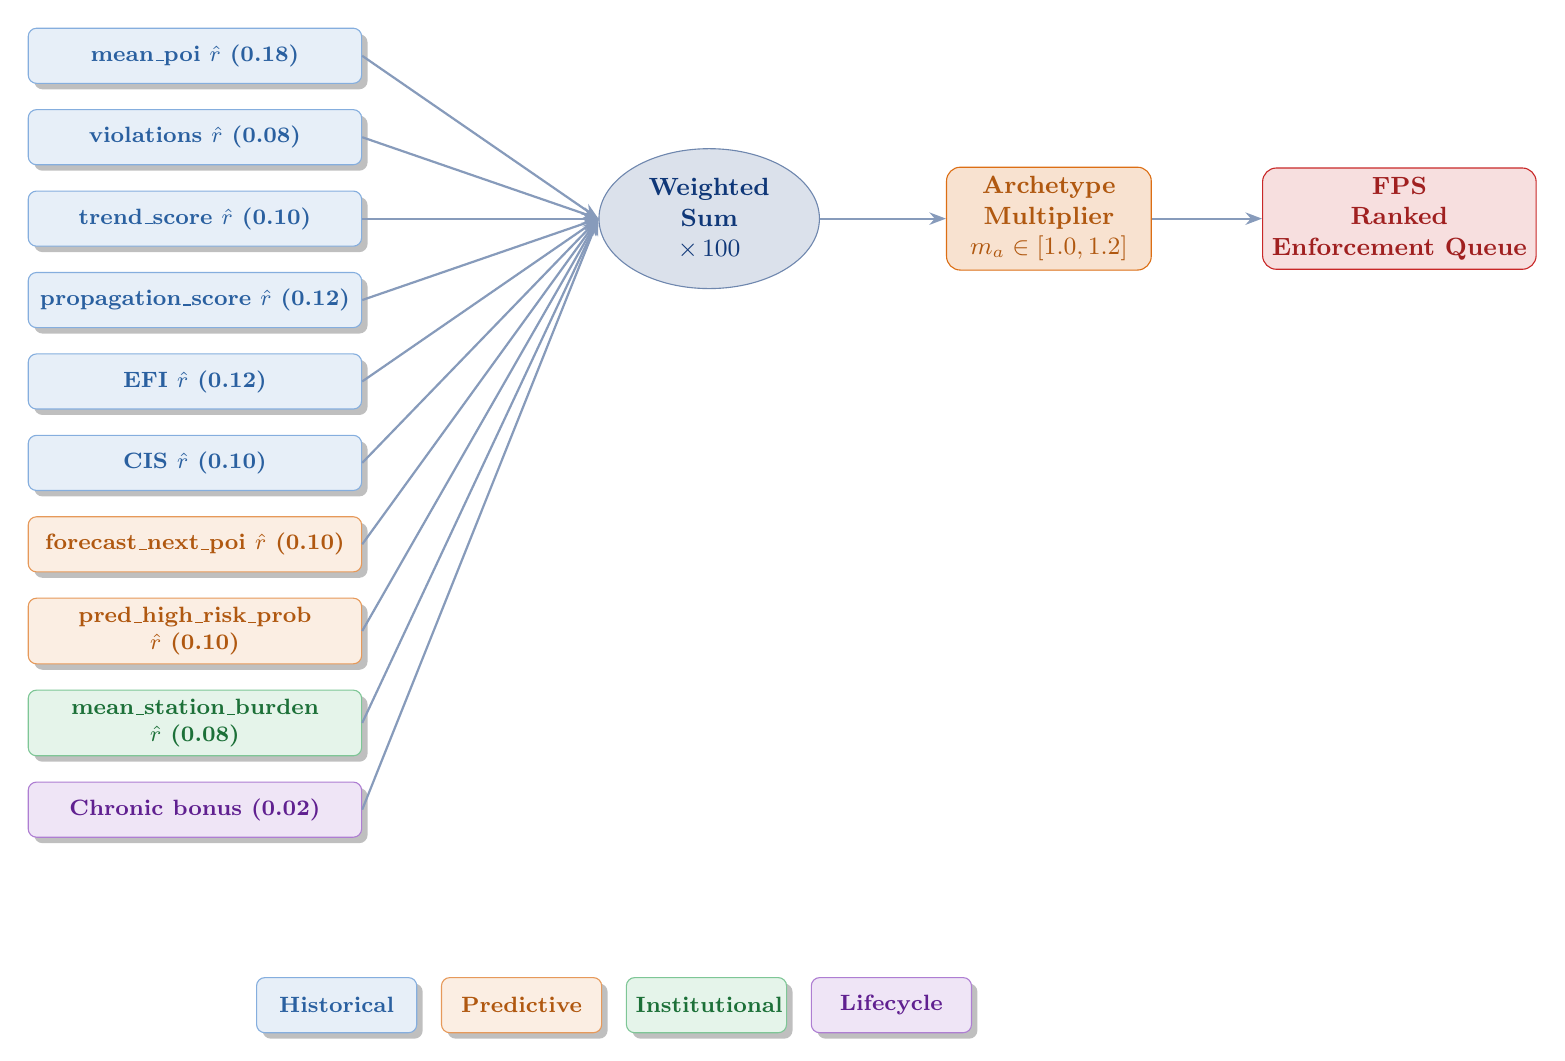
\begin{tikzpicture}[
  node distance = 0.32cm and 1.4cm,
  inpnode/.style  = {rectangle, rounded corners=3pt, minimum width=4.2cm, minimum height=0.7cm,
                 align=center, font=\footnotesize\bfseries, drop shadow, text width=4.0cm},
  histnode/.style = {inpnode, fill=tikzblue!12, draw=tikzblue!60, text=tikzblue!80!black},
  prednode/.style = {inpnode, fill=tikzorange!12, draw=tikzorange!70, text=tikzorange!80!black},
  instnode/.style = {inpnode, fill=tikzgreen!12, draw=tikzgreen!60, text=tikzgreen!70!black},
  bonnode/.style  = {inpnode, fill=tikzpurple!12, draw=tikzpurple!60, text=tikzpurple!80!black},
  rank/.style = {rectangle, rounded corners=5pt, fill=gray!15, draw=gray!60,
                 minimum width=2.5cm, minimum height=1.1cm, align=center,
                 font=\small\bfseries, text=black},
  wsumnode/.style = {ellipse, fill=darkblue!15, draw=darkblue!60, minimum width=2.8cm,
                 minimum height=1.0cm, align=center, font=\small\bfseries, text=darkblue},
  multnode/.style = {rectangle, rounded corners=5pt, fill=tikzorange!20, draw=tikzorange,
                 minimum width=2.6cm, minimum height=0.9cm, align=center,
                 font=\small\bfseries, text=tikzorange!80!black},
  outnode/.style  = {rectangle, rounded corners=5pt, fill=tikzred!15, draw=tikzred,
                 minimum width=3.0cm, minimum height=1.0cm, align=center,
                 font=\small\bfseries, text=tikzred!80!black},
  arr/.style  = {-{Stealth[length=6pt]}, thick, color=darkblue!50},
]

%% --- Historical inputs (col 1, top) ---
\node[histnode] (poi)  {mean\_poi $\hat{r}$ \textbf{(0.18)}};
\node[histnode, below=of poi]  (viol) {violations $\hat{r}$ \textbf{(0.08)}};
\node[histnode, below=of viol] (trnd) {trend\_score $\hat{r}$ \textbf{(0.10)}};
\node[histnode, below=of trnd] (prop) {propagation\_score $\hat{r}$ \textbf{(0.12)}};
\node[histnode, below=of prop] (efi)  {EFI $\hat{r}$ \textbf{(0.12)}};
\node[histnode, below=of efi]  (cis)  {CIS $\hat{r}$ \textbf{(0.10)}};

%% --- Predictive inputs ---
\node[prednode, below=of cis]  (fore) {forecast\_next\_poi $\hat{r}$ \textbf{(0.10)}};
\node[prednode, below=of fore] (risk) {pred\_high\_risk\_prob $\hat{r}$ \textbf{(0.10)}};

%% --- Institutional ---
\node[instnode, below=of risk] (burd) {mean\_station\_burden $\hat{r}$ \textbf{(0.08)}};

%% --- Lifecycle bonus ---
\node[bonnode, below=of burd]  (chro) {Chronic bonus \textbf{(0.02)}};

%% --- Rank + Sum node ---
\node[wsumnode, right=3.0cm of trnd] (wsum) {Weighted\\Sum\\$\times\,100$};

%% --- Archetype multiplier ---
\node[multnode, right=1.6cm of wsum] (mult) {Archetype\\Multiplier\\$m_a \in [1.0,1.2]$};

%% --- Output ---
\node[outnode,  right=1.4cm of mult] (fps) {\textbf{FPS}\\Ranked\\Enforcement Queue};

%% --- Arrows ---
\foreach \n in {poi,viol,trnd,prop,efi,cis,fore,risk,burd,chro} {
  \draw[arr] (\n.east) -- (wsum.west);
}
\draw[arr] (wsum) -- (mult);
\draw[arr] (mult) -- (fps);

%% --- Legend ---
\node[histnode, below=1.2cm of chro, minimum width=2.0cm, text width=1.8cm] (l1) at (1.8,-10.5){Historical};
\node[prednode, right=0.3cm of l1,   minimum width=2.0cm, text width=1.8cm] (l2) {Predictive};
\node[instnode, right=0.3cm of l2,   minimum width=2.0cm, text width=1.8cm] (l3) {Institutional};
\node[bonnode,  right=0.3cm of l3,   minimum width=2.0cm, text width=1.8cm] (l4) {Lifecycle};

\end{tikzpicture}
}
\caption{Priority Engine workflow: ten inputs are percentile-ranked, weighted, summed,
         and post-multiplied by the archetype-specific multiplier to yield the Final
         Priority Score (FPS) and ranked enforcement queue.}
\label{fig:priority_flow}
\end{figure}

%% ============================================================
\subsection{Semantic Search Layer}
%% ============================================================

The Semantic Search Layer enables natural-language querying of the hotspot database—a
capability with no precedent in existing parking enforcement systems.

\paragraph{Text generation.}
Each hotspot row is converted to a structured natural-language description encapsulating
all key scores and categorical labels:
\begin{quote}\small\itshape
``Spatial Cell \{ID\}. Archetype: \{archetype\}. Lifecycle State: \{state\}. Average
Parking Impact Score \{poi\}. Congestion Impact Score \{cis\}. Propagation Score
\{prop\}. Enforcement Failure Index \{efi\}. Priority Score \{fps\}. Recommended
Action: \{action\}.''
\end{quote}

\paragraph{Embedding model.}
Texts are encoded using \texttt{sentence-transformers/all-MiniLM-L6-v2}:
384-dimensional dense vectors, L2-normalised so that cosine similarity reduces to dot
product. GPU-accelerated batch encoding (batch size 64) is the primary pathway; TF-IDF
(max 5,000 features, English stop-word removal) provides a functional fallback.

\paragraph{Retrieval.}
Two retrieval modes are supported:
\begin{enumerate}
  \item \textbf{Cell-to-cell similarity:} $k$-NN ($k=6$, cosine metric) identifies
  the five most similar cells to a query cell, enabling officer generalisation from
  known locations.
  \item \textbf{Free-text query:} The query is encoded by the same model and ranked
  against all cell embeddings by cosine similarity score.
\end{enumerate}


%% ============================================================
\subsection{Graph Analytics Layer}
%% ============================================================

The Graph Analytics Layer models the hotspot ecosystem as a similarity-weighted undirected
graph, enabling identification of structurally central locations whose enforcement yields
network-wide benefits.

\paragraph{Graph construction.}
Each spatial cell is a node. Edges connect cells that are among each other's five nearest
neighbours in the seven-dimensional feature space
$\{\mu_\mathrm{POI}, \text{CIS}, P, \text{EFI}, r_\mathrm{hv}, J_\mu, V\}$.
Edge weight $= 1 - d_\mathrm{cosine}$ (cosine similarity).

\paragraph{Centrality metrics.}

\begin{itemize}
  \item \textbf{PageRank} (weight-informed): identifies cells connected to other
  well-connected, high-severity cells. Enforcing high-PageRank locations produces
  cascading improvements across multiple neighbours.
  \item \textbf{Betweenness Centrality} (weight-informed, normalised): identifies
  gateway cells bridging otherwise disconnected hotspot clusters. Targeted enforcement
  here can fragment the congestion network.
  \item \textbf{Degree:} number of similar cells connected to each node; high degree
  implies the cell represents a common, systematically addressable violation pattern.
\end{itemize}

\paragraph{Community detection.}
Greedy modularity maximisation (Clauset-Newman-Moore) partitions the graph into communities
of co-behaving cells, providing a natural basis for district-level patrol zone assignment
that aligns with the behavioural structure of violations rather than administrative
boundaries.

%% Removed placeholder fig:graph

%% ============================================================
\section{Results and Discussion}

\subsection{Overall Findings}

The analysis of 298,450 parking violations reveals that urban congestion is highly localized and context-dependent. A small fraction of spatial cells is responsible for a disproportionate share of severe traffic disruptions. We discovered that traditional metrics—like raw violation counts—are highly misleading; a single heavy vehicle parked at a major junction generates significantly more network-wide congestion than dozens of two-wheelers on residential side streets. The Parking Obstruction Index (POI) successfully normalizes these disparate events, allowing for objective severity comparison.

Our clustering and propagation models demonstrate that congestion behaves like a network effect. Chronic hotspots rarely exist in isolation; they exhibit significant spillover, degrading traffic flow in adjacent geographic cells. The Enforcement Failure Index (EFI) further highlighted that certain zones are systematically resistant to routine patrols, particularly in overloaded police precincts.

Finally, the archetype discovery phase proved that not all hotspots require the same policing strategy. We identified six distinct behavioral patterns—such as Junction Choke Points and Night Spillovers—that necessitate customized operational responses. By feeding these insights into the CatBoost forecasting model and the multi-component Priority Engine, the platform successfully generated a highly targeted, forward-looking enforcement schedule that optimizes the deployment of limited police resources.

%% ============================================================

\subsection{Dataset Characteristics}

The 298,450 records span 55 police station jurisdictions, 22 vehicle type categories, and
94,412 unique temporal instances. Three columns are entirely null; the enforcement outcome
fields (\texttt{closed\_datetime}, \texttt{action\_taken\_timestamp}) are $100\%$ absent,
confirming that the source system captures initiation events only.

\begin{figure}[htbp]
  \centering
  
\includegraphics[width=\textwidth]{plots/01_missing_values_raw.jpg}
  \caption{Missing value rates bar chart — top 20 columns sorted by missingness percentage}
  \label{fig:miss_bar}
\end{figure}

\subsection{Spatial Distribution of Violations}

The raw geographic scatter reveals pronounced concentration in Bengaluru's central and
south-eastern commercial zones. Transition from raw GPS points to H3-discretised cells
preserves the spatial pattern while eliminating GPS jitter and enabling stable cross-period
comparison.

\begin{figure}[htbp]
  \centering
  
\includegraphics[width=\textwidth]{plots/02_raw_spatial_scatter.jpg}
  \caption{Raw spatial scatter of 298,450 violation coordinates, coloured by POI intensity}
  \label{fig:spatial_scatter}
\end{figure}

\subsection{Temporal Trends}

The hourly violation volume distribution exhibits a bimodal pattern consistent with
Bengaluru's commute schedule: a morning peak and a larger evening peak. Mean POI by hour
amplifies the morning peak—when heavier commercial vehicles are more prevalent—while
night hours (22:00--05:00) account for a minority of violations that are nonetheless
disproportionately severe in profile.

\begin{figure}[htbp]
  \centering
  
\includegraphics[width=\textwidth]{plots/03_hourly_patterns.jpg}
  \caption{Dual panel: hourly violation volume (left) and mean POI by hour (right)}
  \label{fig:temporal}
\end{figure}

\subsection{POI Analysis}

The observed POI distribution (mean~2.586, std~1.504, median~2.245) demonstrates the
right-skewed severity structure expected from a multiplicative composite. The IQR
[1.269, 3.729] encompasses routine violations; the observed maximum of 6.979 confirms
that the most severe violation configurations approach but do not reach the theoretical
ceiling of $\ln(2026) \approx 7.61$.

A notable operational insight: context factors can elevate even a low-weight vehicle to
critical severity. A two-wheeler violation at a chronically active junction in an overloaded
precinct achieves POI $> 4.0$, justifying the same enforcement response as a heavy vehicle
in a less critical context. This context-sensitivity is a deliberate design feature absent
from count-based systems.

\subsection{CIS Analysis}

The CIS distribution approximates uniformity across [0, 100] by construction of the
percentile-rank formulation. The Critical band (CIS $> 75$) identifies the top quartile
of cells by combined congestion impact—the primary enforcement target set for each planning
cycle. Cells with moderate violation counts can achieve Critical CIS through high propagation
scores or enforcement failure, precisely the cases count-based systems would systematically
undervalue.

%% Removed placeholder fig:cis_result

\subsection{Hotspot Discovery Results}

HDBSCAN identifies spatially coherent hotspot clusters across Bengaluru's urban extent.
Noise points are retained in the full pipeline but excluded from cluster quality evaluation.
The Silhouette Coefficient and Davies-Bouldin Index, computed on non-noise points, confirm
that the identified clusters are well-separated and internally compact.

\subsection{Archetype Analysis}

The KMeans archetype model produces six behaviourally distinct cell archetypes. The greedy
label assignment is empirically verified: each archetype's defining characteristic is
maximal within the assigned cluster relative to all others, as confirmed by the cluster
profile heatmap.

\begin{figure}[htbp]
  \centering
  
\includegraphics[width=\textwidth]{plots/07_hotspot_map.jpg}
  \caption{Archetype spatial map — cells colour-coded by archetype, sized by CIS}
  \label{fig:arch_spatial}
\end{figure}

\begin{figure}[htbp]
  \centering
  
\includegraphics[width=\textwidth]{plots/10_archetype_profiles.jpg}
  \caption{Archetype feature profile heatmap — rows = archetypes, columns = 12 cell-level features}
  \label{fig:arch_heat}
\end{figure}

\begin{figure}[htbp]
  \centering
  
\includegraphics[width=\textwidth]{plots/15_top_archetypes.jpg}
  \caption{Archetype distribution bar chart — number of cells per archetype}
  \label{fig:arch_dist}
\end{figure}

\subsection{Forecasting Results}

Table~\ref{tab:forecast} presents the forecasting model evaluation. Exact metric values
are available in the exported \texttt{forecast\_metrics.csv} artifact.

\begin{table}[htbp]
\centering
\caption{Forecasting Model Performance}
\label{tab:forecast}
\begin{tabularx}{\textwidth}{@{}llXXXX@{}}
\toprule
\textbf{Model} & \textbf{Evaluation} & \textbf{MAE} & \textbf{RMSE} & \textbf{Pearson $r$} & \textbf{R$^2$}\\
\midrule
CatBoost (primary)      & Temporal holdout ($t > q_{75}$) & \textit{see artefact} & \textit{see artefact} & \textit{see artefact} & \textit{see artefact}\\
CatBoost (spatial)      & Spatial holdout (20\% cells)    & \textit{see artefact} & \textit{see artefact} & \textit{see artefact} & \textit{see artefact}\\
Mean Baseline           & Temporal holdout                & \textit{see artefact} & \textit{see artefact} & 0.000 & \textit{see artefact}\\
\bottomrule
\end{tabularx}
\end{table}

\paragraph{Metric interpretation.}
MAE measures the mean absolute POI prediction error per hour, directly interpretable in
the POI scale. RMSE penalises large errors more; RMSE materially exceeding MAE indicates
difficult-to-predict extreme events. Pearson $r$ approaching 1.0 confirms directional
reliability even where absolute errors are non-trivial. R$^2$ substantially above 0.0
confirms genuine predictive signal beyond the mean baseline.

The inclusion of cell-level analytical outputs (trend\_score, propagation\_score, EFI,
CIS, archetype\_name) as model features reflects the pipeline's integrated design: the
forecasting module benefits directly from all upstream analytical modules.

\begin{figure}[htbp]
  \centering
  
\includegraphics[width=\textwidth]{plots/12_forecast_eval.jpg}
  \caption{Forecast evaluation: actual vs predicted POI scatter with 45° reference line}
  \label{fig:forecast_scatter}
\end{figure}

%% Removed placeholder fig:forecast_resid

%% Removed placeholder fig:forecast_compare

\subsection{Priority Ranking Results}

The highest-ranked locations are characterised by the intersection of multiple adverse conditions:
high mean POI, Critical CIS, high propagation scores, Chronic lifecycle states, and
assignment to Junction Choke Points ($m_a = 1.20$) or Freight Obstruction Corridors
($m_a = 1.12$). In the ranked output, names such as BTP023 - Mahalaxmi Layout Entrance
(Rajajinagar), BTP083 - AS Char Street, Mysore Road (Chamarajpet), and
BTP204 - ESI Hospital, Rajajinagar appear at the top because they combine structural
junction pressure with high propagation and persistent enforcement demand. The ten-component
priority engine prevents any single extreme value from dominating the ranking—a location
must perform adversely across multiple dimensions to achieve top position.

\begin{figure}[htbp]
  \centering
  \includegraphics[width=\textwidth]{plots/top_hotspots_named.jpg}
  \caption{Top hotspots by Final Priority Score - human-readable location labels}
  \label{fig:top15}
\end{figure}

\begin{figure}[htbp]
  \centering
  
\includegraphics[width=\textwidth]{plots/11_trend_propagation_failure.jpg}
  \caption{Enforcement priority spatial map — all cells sized by violation count, coloured by FPS}
  \label{fig:priority_map}
\end{figure}

\subsection{Semantic Search Results}

For the sample query \textit{``junction choke point with chronic parking and spillover''}, the
top-$N$ results consistently retrieve cells assigned to the Junction Choke Points archetype
with Chronic or Emerging lifecycle states and high propagation scores—confirming that the
MiniLM-L6-v2 embedding model has captured the semantic structure of the hotspot descriptions.

%% Removed placeholder fig:sem_map

\subsection{Graph Analytics Results}

The hotspot similarity graph exhibits a power-law-like degree distribution: a small number
of cells accumulate high degree through similarity connections to many others. PageRank
identifies cells whose influence extends beyond their immediate neighbourhood—the strategically
optimal targets for enforcement that produces network-wide congestion reduction.

Betweenness centrality reveals gateway cells positioned between otherwise weakly connected
regions. Targeting these cells can decouple previously interconnected congestion zones.
Community detection partitions the graph into coherent super-clusters aligning with the
behavioural archetype structure, providing a natural basis for district-level resource
allocation. In the current graph, \textbf{Devanahalli Airport} is the highest PageRank node,
which shows that some centrally connected locations matter for coordination even when they
are not the highest-priority enforcement sites.

\begin{figure}[htbp]
  \centering
  
\includegraphics[width=\textwidth]{plots/13_graph_analytics.jpg}
  \caption{Graph degree distribution histogram}
  \label{fig:degree}
\end{figure}

%% Removed placeholder fig:pagerank_cis

%% ============================================================
\section{Operational Impact}
%% ============================================================

The Parking Operational Intelligence Platform moves Bengaluru Traffic Police from a reactive, count-based policing model to a proactive, intelligence-driven enforcement strategy. 

\subsection{Daily Enforcement and Pre-Positioning}
The \texttt{priority\_table} provides a pre-sorted, annotated dispatch schedule. Instead of randomly patrolling sectors, officers are directed to the highest-impact cells first. Furthermore, the \texttt{forecast\_next\_poi} predictions enable anticipatory patrol positioning—allowing commanders to deploy tow vehicles at projected choke points before the violations actually accumulate into gridlock.

\subsection{Archetype-Specific Interventions}
The system replaces generic patrols with tailored enforcement protocols based on the discovered behavioral archetypes:

\begin{itemize}[leftmargin=1.5em]
  \item \textbf{Junction Choke Points:} 
  These locations experience severe intersection blockages that suppress multiple traffic flows simultaneously. Traffic police should increase physical patrol presence exclusively during morning and evening peak hours. Towing vehicles must be kept on immediate standby in these cells, and rapid-response motorcycle units should be utilized to quickly clear blockages before spillover occurs.
  
  \item \textbf{Night Spillovers:} 
  Characterized by parking overflow between 22:00 and 05:00 adjacent to nightlife and dining districts. Enforcement should shift from physical patrols to camera-assisted monitoring and automated ticketing. Police should also coordinate with nearby commercial establishments to manage valet parking effectively and prevent lane obstruction.
  
  \item \textbf{Freight Obstruction Corridors:} 
  These are arterial routes blocked by trucks and lorries during commercial loading. The operational response requires restricting loading/unloading entirely during peak commuter hours. Officers should enforce strict, designated freight windows and aggressively target commercial vehicles that violate these temporal boundaries.
  
  \item \textbf{Weekend Event Zones:} 
  These areas are well-managed during the week but overwhelmed on weekends due to localized events. Police should deploy temporary barricades to physically prevent illegal parking. Event-based marshals should be scheduled dynamically based on the venue's calendar, and dynamic parking restrictions should be enforced using mobile signage.
\end{itemize}

%% ============================================================
\subsection{Policy Recommendations}
%% ============================================================

To fully leverage the insights generated by this platform, the following smart-city policy interventions are recommended for the Bengaluru Traffic Police and municipal authorities. The policy layer is intentionally practical: it can plug into Bengaluru-style traffic command centres and ICCC-style dashboards, and it follows the logic behind demand-responsive parking systems such as SFpark, where parking controls adapt to demand instead of remaining static.

\begin{enumerate}[leftmargin=1.5em]
  \item \textbf{Dynamic Enforcement Scheduling:} Transition away from static patrol shifts. Align officer deployment schedules directly with the temporal peaks identified by the forecasting engine.
  \item \textbf{Data-Driven Patrol Allocation:} Allocate towing fleets and personnel across precincts proportionally based on the Congestion Impact Score (CIS) rather than geographic area or historical precedent.
  \item \textbf{Temporary No-Parking Zones:} Utilize the archetype analysis to define dynamic, time-bound parking restrictions (e.g., restricted parking only on weekends or only during night hours).
  \item \textbf{Freight Movement Regulations:} Implement city-wide policy restricting commercial loading on identified Freight Obstruction Corridors during the 07:00--10:00 and 17:00--21:00 windows.
  \item \textbf{Junction Protection Policies:} Establish strict zero-tolerance zones extending 50 meters from any cell classified as a Junction Choke Point, enforced via automated cameras.
  \item \textbf{Event-Based Traffic Planning:} Mandate large commercial venues in Weekend Event Zones to submit traffic management plans and fund auxiliary traffic marshals during peak operational days.
  \item \textbf{Congestion Early-Warning Systems:} Integrate the 1-hour CatBoost forecast directly into the police control room dispatch software to trigger automated alerts when a cell's risk probability exceeds 90\%.
  \item \textbf{Smart-City Dashboard Integration:} Pipe the exported GeoJSON hotspot layers and Priority Queue into Bengaluru's existing Integrated Command and Control Centre (ICCC) for unified urban management.
\end{enumerate}

%% ============================================================
\section{Limitations}
%% ============================================================

While the platform introduces significant advancements in spatial intelligence, several limitations remain. The current architecture relies on batch processing of static datasets, whereas production deployment would require streaming integration for incremental score updates. Spatial propagation is modelled using Euclidean distance rather than road-network distance, which may misrepresent spillover effects along one-way or curved segments. Furthermore, the forecasting module is restricted to single-step hourly predictions and lacks external contextual data such as real-time traffic speeds, weather conditions, or transit disruptions. Analytically, the KMeans clustering model enforces hard assignments that may misclassify boundary cells, and the complete absence of closed-loop enforcement outcome data prevents direct empirical validation of the priority ranking's effectiveness.


%% ============================================================
\section{Future Work}
%% ============================================================

Future iterations of the platform should transition to a real-time, event-driven architecture using streaming pipelines to enable dynamic, shift-level priority updates. The spatial propagation model can be enhanced by integrating OpenStreetMap routing graphs to compute true network-distance-weighted spillover. Methodologically, Graph Neural Networks (such as GCN or GraphSAGE) could replace hand-engineered features with learned spatial representations, and spatio-temporal GNNs could enable robust, multi-horizon joint forecasting. Operationally, reinforcement learning could be utilized to develop adaptive patrol policies that optimize fleet allocation, while the integration of multimodal sensing—such as CCTV feeds and municipal event calendars—would significantly enrich the system's contextual awareness and predictive accuracy.


%% ============================================================
\section{Conclusion}
%% ============================================================

This paper has presented the Parking Operational Intelligence Platform—a comprehensive
AI-driven framework that addresses the fundamental limitation of existing parking enforcement
systems: the inability to translate raw violation records into systematic, prioritised, and
actionable enforcement intelligence.

The central methodological contribution is a multi-layer analytical pipeline operating
across four complementary dimensions: (1) \textbf{severity} through the seven-factor
multiplicative Parking Obstruction Index (POI, observed range [0.318, 6.979]); (2)
\textbf{spatial network effects} through the distance-weighted propagation score; (3)
\textbf{institutional capacity} through the Enforcement Failure Index; and (4)
\textbf{network-wide congestion impact} through the Congestion Impact Score with
interpretable quartile banding (Low / Medium / High / Critical).

Beyond these core metrics, the system introduces a six-state hotspot lifecycle taxonomy, a
data-driven six-archetype behavioural classification with tailored intervention strategies, a
ten-component priority engine with archetype-specific multipliers (1.00--1.20), a
transformer-based semantic search layer, and a PageRank-based graph intelligence module.

The final system output is a production-ready, multi-format dashboard comprising a ranked
enforcement queue, interactive geospatial visualisation, GeoJSON export, semantic hotspot
index, and graph analytics summary—all derived from a single execution of the analytical
pipeline on 298,450 raw violation records from Bengaluru.

The POIP system demonstrates that raw parking violation data, when subjected to principled
multi-dimensional feature engineering and integrated analytical modelling, yields far richer
enforcement intelligence than any single-metric approach can provide. Its modular,
interpretable architecture provides a foundation for real-time streaming integration, graph
neural network enhancement, and reinforcement-learning-based patrol optimisation in future
iterations.

\end{document}
